%%%%%%%%%%%%%%%%%%%%%%%%%%%%%%%%%%%%%%%%%%%%%%%%%%%%%%%%%%%%%%
%% Chapter 4: Isolated Gloss Recognition (video2gloss)
%%%%%%%%%%%%%%%%%%%%%%%%%%%%%%%%%%%%%%%%%%%%%%%%%%%%%%%%%%%%%%

\section{Isolated Gloss Recognition (video2gloss)}
\label{chap:isolated-gloss-recognition}

To address the video-to-gloss task introduced in
Chapter~\ref{chap:related-work}, we adopt a retrieval-based paradigm: rather
than learning a fixed set of class boundaries, we learn an embedding space in
which examples of the same gloss cluster together, and defer classification to
nearest-neighbour retrieval within that space
(Figure~\ref{fig:slt-problem-overview}). This formulation handles intra-class
spread more gracefully than a softmax classifier, scales naturally to new
vocabulary without retraining the classifier head, and provides a
representational backbone amenable to the alignment-based and
continuous-recognition extensions discussed in
Section~\ref{sec:gloss-recognition-discussion}.

\begin{figure}[htbp]
  \centering
  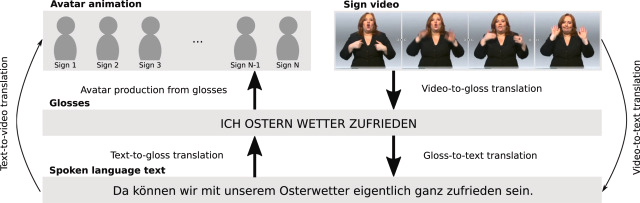
\includegraphics[width=0.85\textwidth]{figures/gloss-recognition/slt-problem-overview.png}
  \caption{The general problem of sign language translation and the position of
  the video-to-gloss task within it.}
  \label{fig:slt-problem-overview}
\end{figure}

This chapter's contributions are: (i) a retrieval-based formulation of isolated
video-to-gloss recognition, casting gloss recognition as metric learning
followed by nearest-neighbour retrieval; (ii) a multi-objective training scheme
combining a Multi-Similarity metric learning loss with an auxiliary
landmark-reconstruction objective; (iii) a controlled benchmark of five temporal
encoders -- Transformer, LSTM, BiLSTM, GRU, and BiGRU -- under identical
preprocessing, sampling, loss, and training configurations; and (iv) a geometric
characterisation of the signer-variability problem via confusion-matrix
analysis, per-class recall, t-SNE visualisation, and positive/negative pair
distance tracking.

\subsection{Dataset and preprocessing}
\label{sec:gloss-recognition-dataset}

The experiments presented in this chapter are conducted on a subset of the ASL
Citizen dataset (Microsoft, 2023), a large-scale American Sign Language corpus
collected with an emphasis on signer diversity and ecological validity. The full
dataset comprises 1{,}068 annotated sign videos spanning a broad lexical range.
For benchmarking, a subset of 32 glosses was selected, chosen to cover a
representative variety of semantic categories -- everyday objects, actions,
temporal expressions, colours, and social roles:

\begin{quote}
\small
BASKETBALL, BEE, BREAKFAST, CALL, CAR, CAT, CHRISTMAS, DEAF, DOG, EAT, FIREMAN,
FISH, FOOTBALL, GREEN, HEAD, HOSPITAL, KID, LUNCH, MAN, MECHANIC, MORNING,
NIGHT, NO, NOON, RED, SMILE, STUDENT, TRIP, UNIVERSITY, VALUE, WOMAN, YES.
\end{quote}

\label{sec:gloss-recognition-preprocessing}
The preprocessing pipeline operates not on raw video but on the per-frame
landmark sequences extracted by MediaPipe, as produced by the annotation
platform described in Section~\ref{sec:annotation-data-format}. Each frame is
represented as a 144-dimensional vector comprising a selected subset of
upper-body pose landmarks together with the full left- and right-hand landmark
sets. MediaPipe operates on a per-frame basis, producing coordinates for a set
of anatomically well-defined body landmarks -- including joints such as wrists,
knuckles, and finger tips -- each reported as a 3D position relative to a
designated anatomical reference point: the hip centre for body pose, and the
wrist for hand landmarks (Figure~\ref{fig:mediapipe-intuition} and
Figure~\ref{fig:mediapipe-holistic-landmarks}). Operating on landmark sequences
rather than raw video frames promotes generalisation across signers by
abstracting away appearance-level variation such as skin tone, clothing, and
lighting, and directs the model's attention toward the signal most relevant to
sign language: structured human body motion over time.

\begin{figure}[htbp]
  \centering
  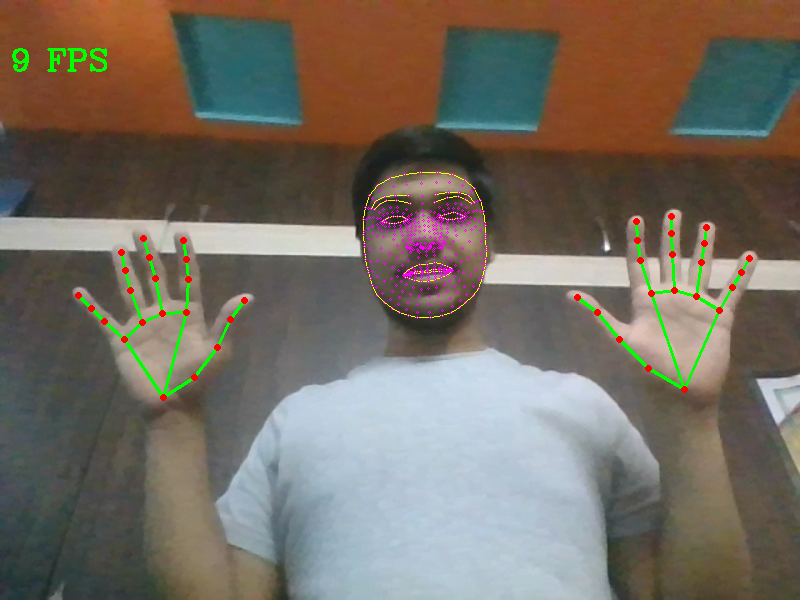
\includegraphics[width=0.85\textwidth]{figures/gloss-recognition/mediapipe-intuition.png}
  \caption{Intuition behind MediaPipe landmark extraction.}
  \label{fig:mediapipe-intuition}
\end{figure}

\begin{figure}[htbp]
  \centering
  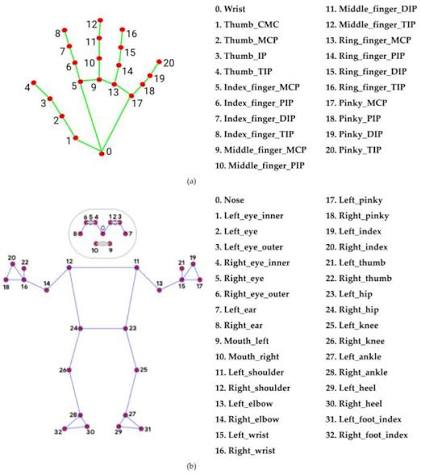
\includegraphics[width=0.7\textwidth]{figures/gloss-recognition/mediapipe-holistic-landmarks.png}
  \caption{MediaPipe Holistic landmark layout (pose, face, and hands).}
  \label{fig:mediapipe-holistic-landmarks}
\end{figure}

The preprocessing pipeline proceeds through the following stages:

\begin{enumerate}
  \item \textbf{Hand activity check} -- hand presence is assessed across the
        full sequence; if a given hand is absent for the majority of frames,
        its landmark coordinates are replaced with the position of the
        corresponding shoulder joint for those frames. This provides the model
        with a stable, anatomically grounded placeholder rather than exposing
        it to a largely missing coordinate track, which could otherwise
        introduce spurious gradients or corrupt temporal interpolation;
  \item \textbf{Temporal interpolation} -- landmark coordinates missing for
        isolated frames (but not for the majority of the sequence) are
        recovered via linear interpolation along the time axis; coordinate
        tracks missing entirely, and therefore not interpolable, are filled
        with zero;
  \item \textbf{Static frame removal} -- frames contributing negligible motion
        are identified and discarded by thresholding the frame-to-frame
        landmark displacement magnitude, focusing the temporal encoder on
        gesture-relevant dynamics;
  \item \textbf{Smoothing} -- the remaining sequence is smoothed using a
        Savitzky-Golay filter, suppressing high-frequency landmark jitter
        arising from MediaPipe detection noise while preserving the underlying
        motion trajectory;
  \item \textbf{Spatial normalisation} -- landmark coordinates are normalised
        by translating the origin to the midpoint between the two shoulders and
        rescaling by the inter-shoulder distance, rendering the representation
        invariant to the signer's absolute position and physical scale within
        the frame;
  \item \textbf{Temporal resampling} -- every preprocessed sequence is resampled
        to a fixed length of 60 frames via interpolation, ensuring uniform
        input length across all samples regardless of the original recording
        duration.
\end{enumerate}

\subsection{Model architecture}
\label{sec:gloss-recognition-model}

Given a full recording of a sign gesture, each frame is processed using
MediaPipe to extract skeletal landmarks covering the human pose, hands, and
face. To achieve pose-invariant representations and eliminate dependence on
absolute body position within the frame, the landmark coordinates are
normalised and each per-frame landmark set is flattened into a continuous
vector $\mathbb{R}^L$, where $L$ denotes the total number of landmark
coordinates. Flattening discards the explicit topological structure of the
skeletal graph -- the anatomical connectivity between landmarks (e.g.\ that the
wrist is the parent joint of the metacarpals) -- so the model must implicitly
infer any spatial relationships between landmarks rather than having them
structurally encoded; this limitation is revisited in
Section~\ref{sec:gloss-recognition-discussion}.

The resulting sequence of frame-level vectors is first projected into a
higher-dimensional space via a time-distributed linear layer -- a single dense
layer applied independently and identically at each timestep -- and then passed
to a temporal encoder, which may be instantiated as a Transformer, LSTM, GRU,
BiLSTM, or BiGRU (Figure~\ref{fig:model-architecture}). The encoder operates
across the full temporal extent of the sequence, producing a sequence of
temporally contextualised embeddings, one per input frame.

\begin{figure}[htbp]
  \centering
  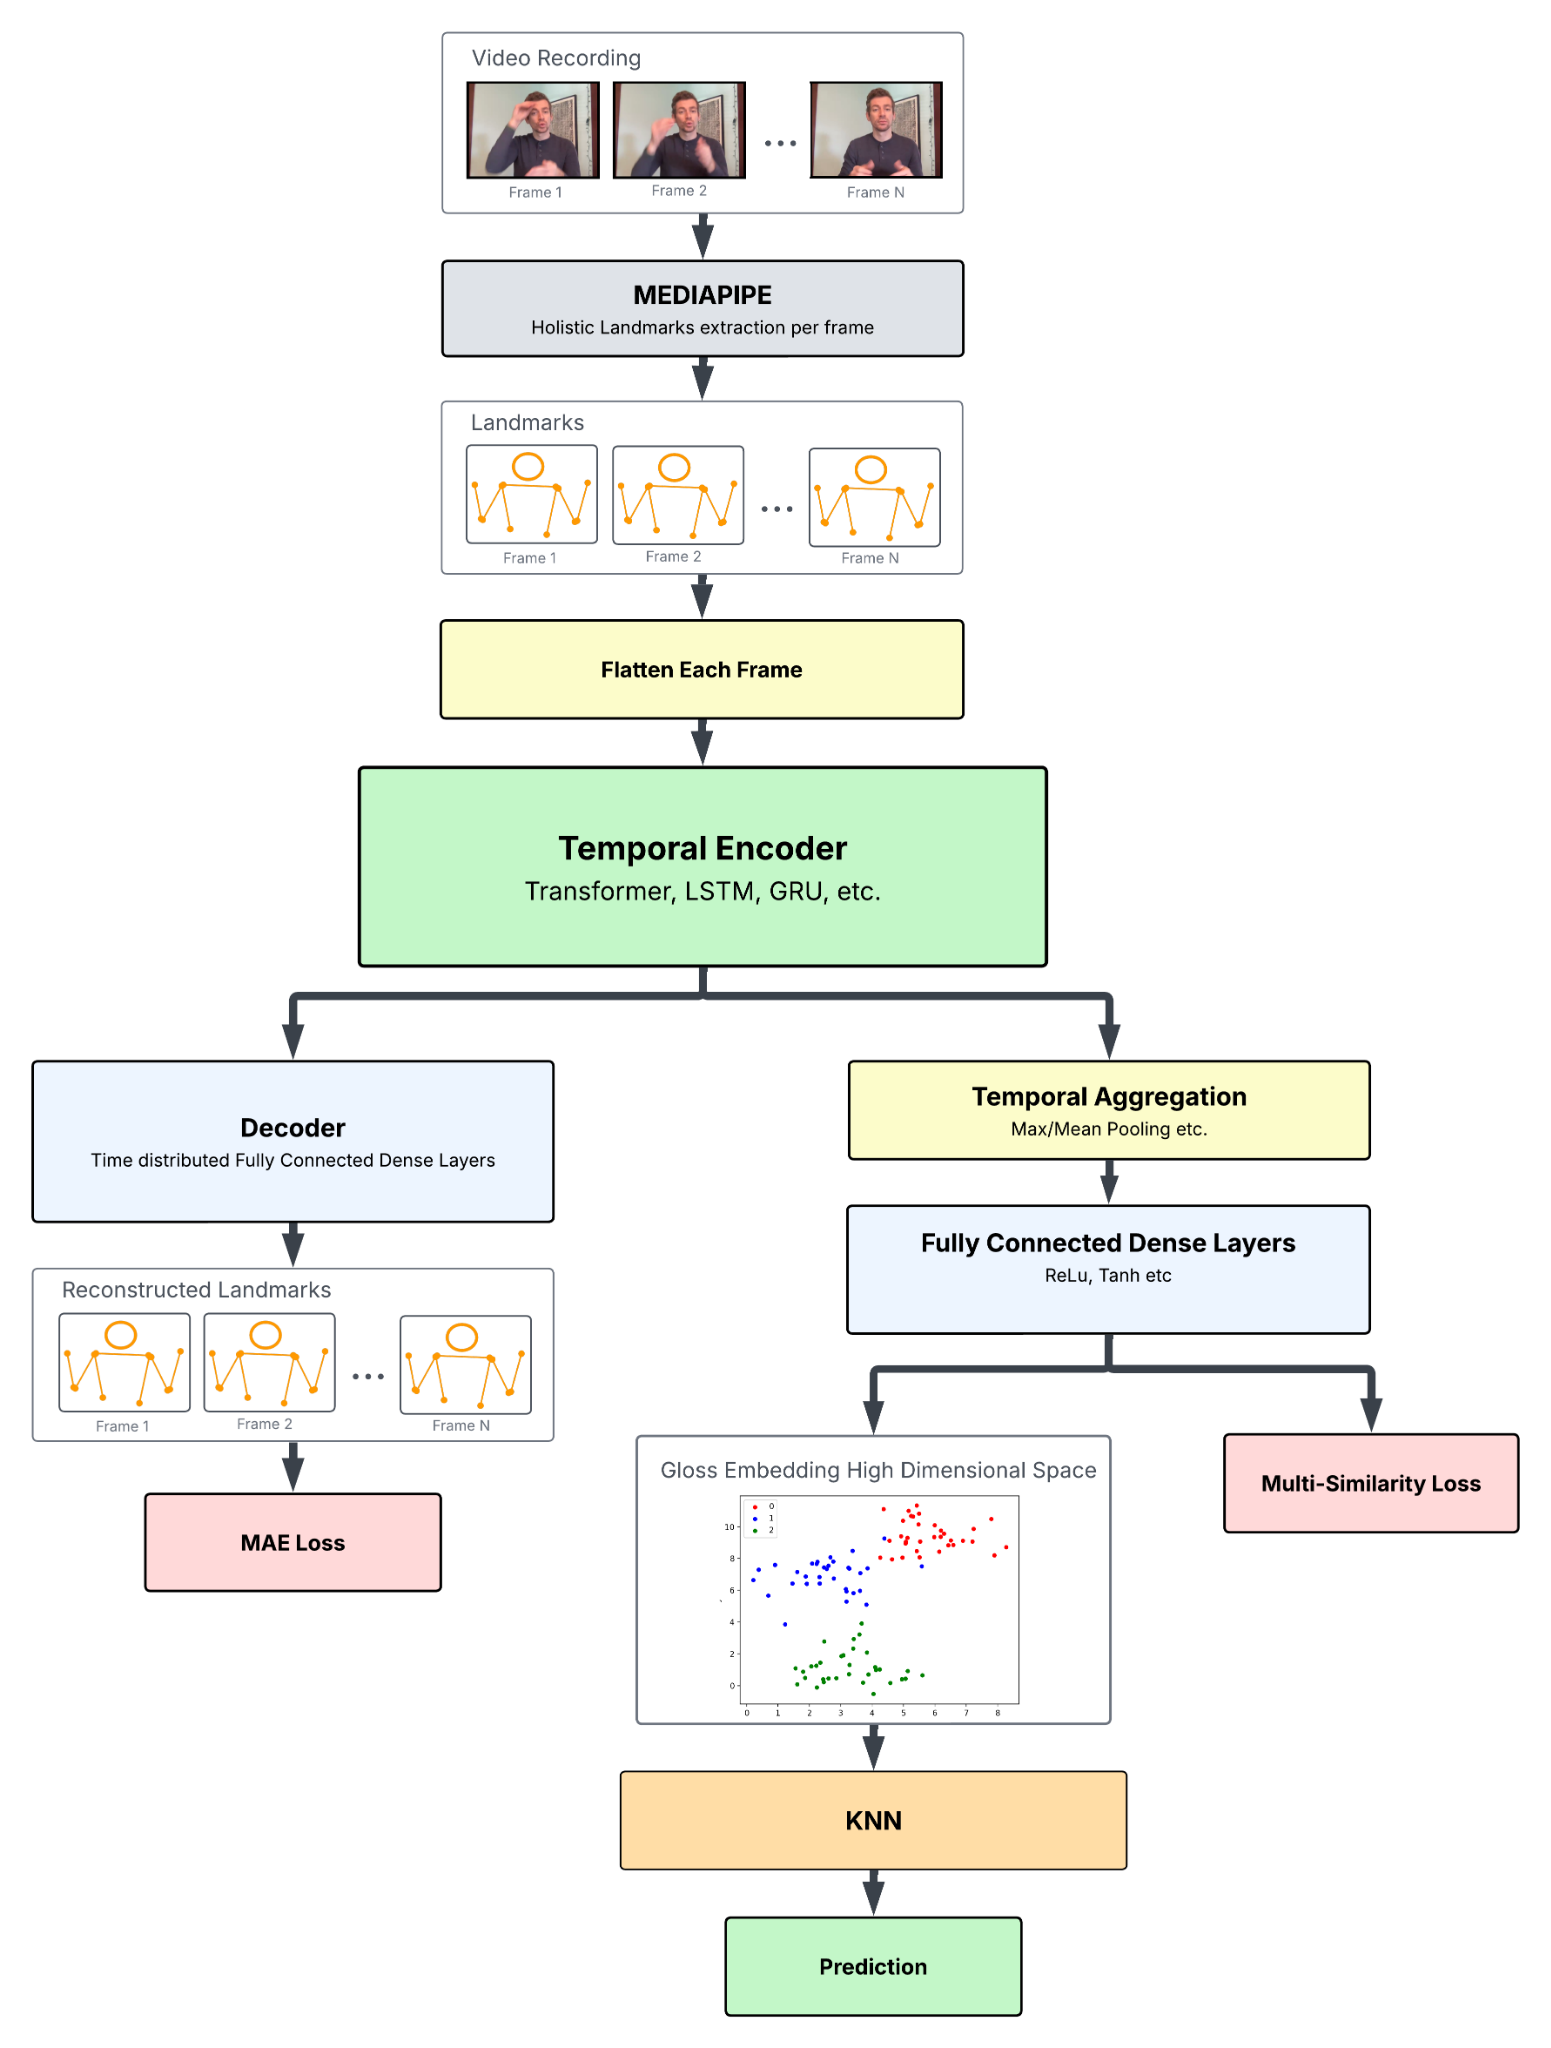
\includegraphics[width=0.85\textwidth]{figures/gloss-recognition/model-architecture.png}
  \caption{General architecture of the proposed retrieval-based video-to-gloss
  recognition model.}
  \label{fig:model-architecture}
\end{figure}

\subsubsection{Temporal encoders}

The LSTM encoder processes the input sequence autoregressively in the forward
temporal direction (Figure~\ref{fig:lstm-cell}). At each timestep $t$, the LSTM
cell takes the current projected embedding $x_t$ alongside the hidden state
$h_{t-1}$ and cell state $c_{t-1}$ carried over from the previous step, and
produces an updated hidden state $h_t$. The cell state acts as a long-range
memory mechanism, allowing the network to selectively retain or discard
information across arbitrarily distant timesteps via its gating structure. The
BiLSTM extends this by running two independent LSTM chains over the same
sequence, one forward and one in reverse, concatenating their outputs at each
position $t$ into a unified hidden state $h_t = [h_t^{\rightarrow};
h_t^{\leftarrow}]$, thus capturing both past and future context relative to
that position.

\begin{figure}[htbp]
  \centering
  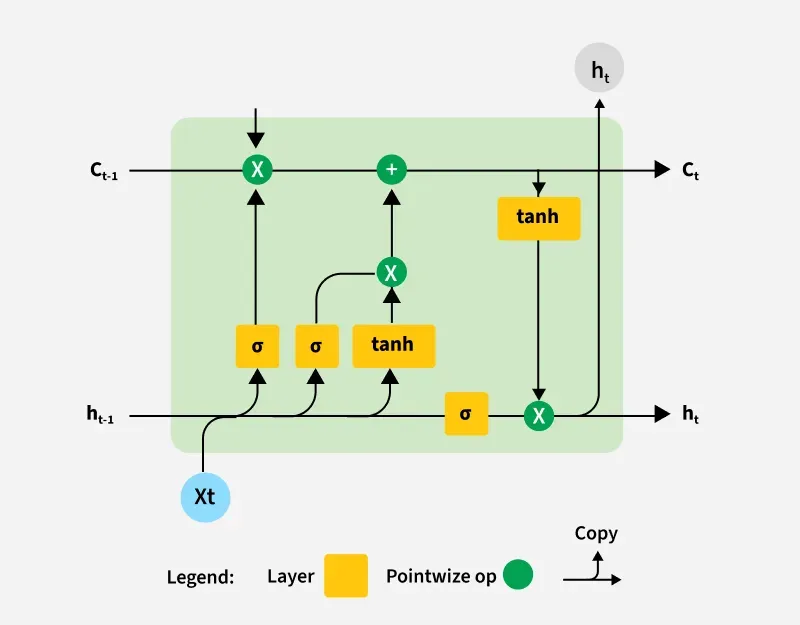
\includegraphics[width=0.6\textwidth]{figures/gloss-recognition/lstm-cell.png}
  \caption{LSTM cell (left) and its bidirectional extension, BiLSTM (right).}
  \label{fig:lstm-cell}
\end{figure}

The GRU encoder similarly processes the input sequence in the forward temporal
direction, but simplifies the LSTM cell by replacing the separate hidden and
cell states with a single unified hidden state $h_t$ (Figure~\ref{fig:gru-cell}).
Rather than an input gate, forget gate, and output gate, the GRU employs an
update gate $z_t$, controlling how much of the previous hidden state is carried
forward, and a reset gate $r_t$, determining how much prior context influences
the candidate hidden state. This reduced parameterisation makes the GRU
computationally lighter than the LSTM while retaining its capacity to model
long-range temporal dependencies. The BiGRU follows the same extension
principle as the BiLSTM, running two independent GRU chains over the sequence in
opposite directions and concatenating their outputs at each timestep.

\begin{figure}[htbp]
  \centering
  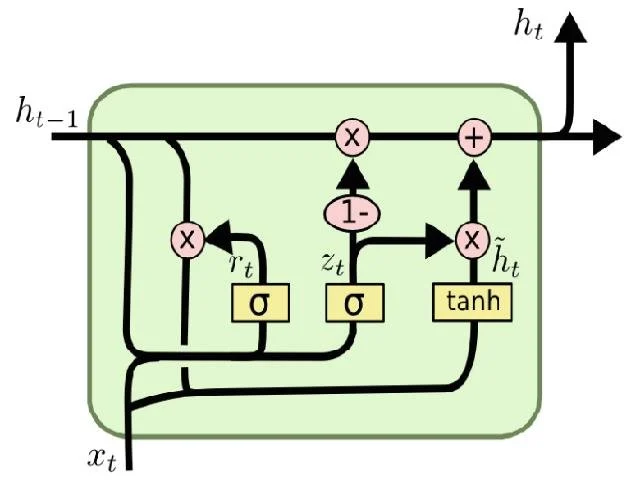
\includegraphics[width=0.6\textwidth]{figures/gloss-recognition/gru-cell.png}
  \caption{GRU cell (left) and its bidirectional extension, BiGRU (right).}
  \label{fig:gru-cell}
\end{figure}

The Transformer encoder departs fundamentally from the recurrent paradigm: it
operates on all timesteps in parallel rather than step by step
(Figure~\ref{fig:transformer-encoder}). Because the architecture is inherently
permutation-invariant, explicit positional encodings are added to the projected
input embeddings prior to processing. The core computational unit is scaled
dot-product self-attention: at each layer, every position $t$ computes a query
$q_t$, a set of keys $\{k_1, \ldots, k_T\}$, and a set of values
$\{v_1, \ldots, v_T\}$ via learned linear projections of the input, and the
output at position $t$ is a weighted sum of all value vectors, where the weight
assigned to position $s$ is proportional to
$\exp(q_t^\top k_s / \sqrt{d_k})$, with $d_k$ the key dimensionality. Every
position therefore attends directly to every other position in a single layer,
giving the Transformer a global receptive field from the first layer -- a
property neither LSTM nor GRU possesses without depth. Self-attention is
computed across $H$ independent heads in parallel, with their outputs
concatenated and linearly projected; each self-attention sublayer is followed by
a position-wise feed-forward network, with residual connections and layer
normalisation wrapping both sublayers.

\begin{figure}[htbp]
  \centering
  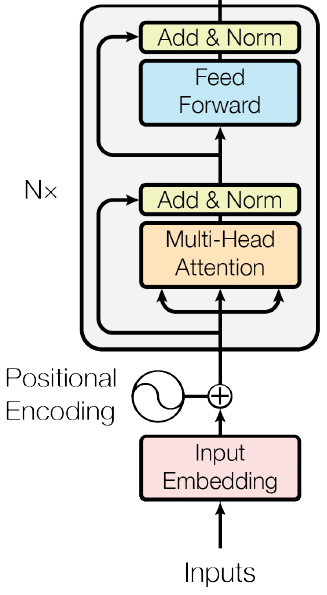
\includegraphics[width=0.6\textwidth]{figures/gloss-recognition/transformer-encoder.png}
  \caption{Transformer encoder.}
  \label{fig:transformer-encoder}
\end{figure}

\subsubsection{Reconstruction decoder, aggregation, and retrieval}

The encoder output is routed through two parallel branches. The first, a
reconstruction decoder -- a stack of time-distributed dense layers -- attempts
to recover the original per-frame landmark vectors from their encoded
representations. This auxiliary objective serves as a regularisation mechanism:
by requiring the encoder to retain sufficient information to reconstruct its
input, it discourages representational collapse and encourages the learning of
dense, geometrically faithful embeddings. Critically, this also lays the
groundwork for a planned extension of the retrieval pipeline: because the
learned embeddings remain grounded in the structure of the original landmark
space, they are well-suited to Dynamic Time Warping (DTW)-based sequence
alignment, discussed further in Section~\ref{sec:gloss-recognition-discussion}.

The second branch applies temporal aggregation -- Global Mean Pooling across the
temporal dimension of the encoder output, computing the elementwise mean over
all $T$ timesteps to produce a single fixed-length vector $z \in \mathbb{R}^d$ --
followed by a stack of fully connected dense layers that project $z$
non-linearly into a high-dimensional embedding space. This final projection does
not itself produce a classification decision; rather, its output is a
continuous embedding vector that serves as the input domain for a $k$-nearest
neighbours (KNN) classifier. The dense layers are thus trained not to
discriminate directly between gloss classes, but to shape the geometry of the
embedding space such that embeddings of the same gloss cluster tightly together
while embeddings of distinct glosses are pushed apart. Classification is
delegated entirely to KNN, which retrieves the $k$ most similar embeddings from
a labelled reference set and determines the predicted gloss by majority vote
over their labels.

\subsubsection{Composite loss}

To impose the desired geometric structure on the embedding space, we adopt the
Multi-Similarity (MS) loss \cite{wang2019msloss} as the metric learning
objective. Unlike simpler contrastive or triplet losses, which consider only
individual pairs or triplets in isolation, the MS loss operates on the full
pairwise similarity structure within a training batch. For each anchor
embedding $i$, it defines a set of positive pairs $P_i$ (embeddings sharing the
same gloss label) and a set of negative pairs $N_i$ (embeddings of distinct
glosses), and applies asymmetric soft-weighting to both sets based on pairwise
cosine similarities $S_{ik}$:

\begin{equation}
  \mathcal{L}_{MS} = \frac{1}{m}\sum_{i=1}^{m}\left\{
    \frac{1}{\alpha}\log\!\left[1+\sum_{k\in P_i}e^{-\alpha(S_{ik}-\lambda)}\right]
  + \frac{1}{\beta}\log\!\left[1+\sum_{k\in N_i}e^{\beta(S_{ik}-\lambda)}\right]
  \right\}
  \label{eq:ms-loss}
\end{equation}

where $\alpha$ and $\beta$ are scaling hyperparameters controlling the
steepness of the positive and negative weighting respectively, and $\lambda$ is
a margin threshold. The combined effect is to pull same-gloss embeddings
together while pushing distinct-gloss embeddings apart, with gradient signal
concentrated on the most discriminatively useful pairs in each batch.

The MS loss is combined additively with the Mean Squared Error (MSE)
reconstruction loss produced by the decoder branch, penalising deviation
between the original per-frame landmark vectors $x_t$ and their
reconstructions $\hat{x}_t$:

\begin{equation}
  \mathcal{L}_{rec} = \frac{1}{T}\sum_{t=1}^{T} \lVert x_t - \hat{x}_t \rVert_2^2
  \label{eq:mse-loss}
\end{equation}

The two objectives are combined into a composite loss via a scalar weighting
hyperparameter $\gamma$, which governs the relative contribution of the
reconstruction term:

\begin{equation}
  \mathcal{L} = \mathcal{L}_{MS} + \gamma\, \mathcal{L}_{rec}
  \label{eq:composite-loss}
\end{equation}

\subsection{Experiments and results}
\label{sec:gloss-recognition-experiments}

\subsubsection{Training procedure}

The model is trained as a metric learning encoder whose objective is to produce
a geometrically structured embedding space over gesture representations. All
embeddings are L2-normalised prior to both loss computation and evaluation,
constraining the embedding space to the unit hypersphere and ensuring that
cosine similarity and Euclidean distance are equivalent metrics.

Training uses the Adam optimiser with an initial learning rate of
$5\times10^{-4}$, following a Cosine Annealing with Warm Restarts schedule
($T_0=30$, $T_{mult}=2$, $\eta_{min}=1\times10^{-6}$;
Figure~\ref{fig:lr-schedule}), in which the learning rate decays along a cosine
curve from its current maximum to $\eta_{min}$, then periodically restarts at a
higher value, with the restart interval doubling after each cycle. Training
batches are constructed using a $P \times K$ sampler with $P=16$ classes and
$K=4$ samples per class, yielding batches of up to 64 samples -- a
class-balanced sampling strategy that is a prerequisite for effective metric
learning, ensuring each batch contains sufficient positive and negative pairs
for the MS loss to produce informative gradients. The composite loss weight was
set to $\gamma=0.25$, allowing the reconstruction term to regularise the
encoder without dominating the metric learning objective.

\begin{figure}[htbp]
  \centering
  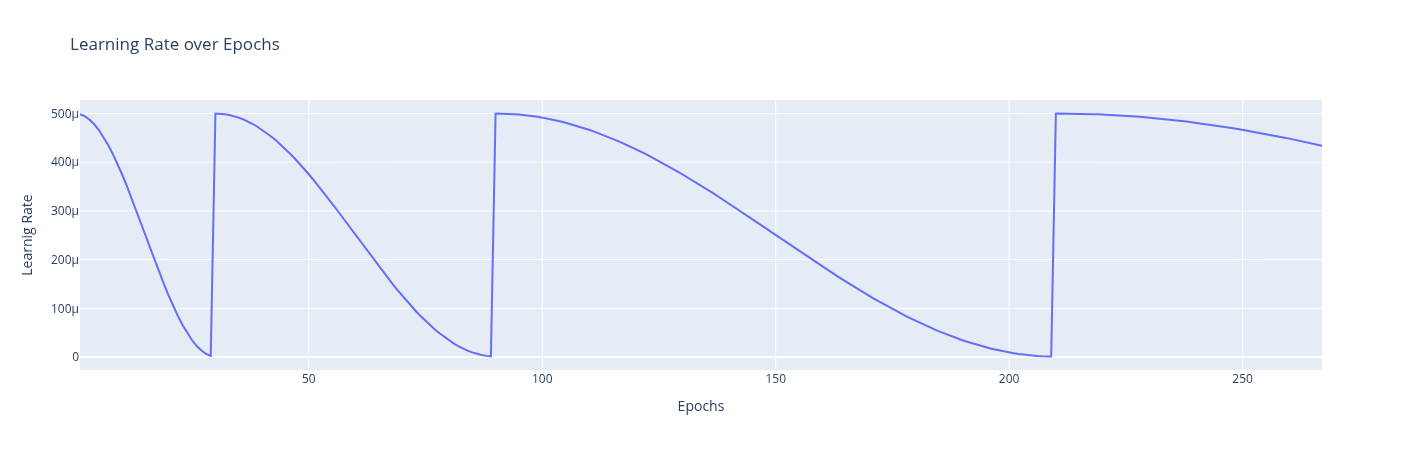
\includegraphics[width=0.65\textwidth]{figures/gloss-recognition/lr-schedule.png}
  \caption{Learning rate schedule over the course of training.}
  \label{fig:lr-schedule}
\end{figure}

Beginning at epoch 30, an Exponential Moving Average (EMA) of the model weights
is maintained with a decay coefficient of 0.99; from this point onward, the EMA
model is used exclusively for validation and checkpointing in place of the raw
parameter snapshot, typically yielding more stable and generalisable evaluation
performance. Model performance is evaluated on the validation set using
1-nearest-neighbour (1-NN) accuracy in the learned embedding space -- each
validation sample is assigned the label of its single nearest neighbour in the
embedding space constructed from the training set. The checkpoint attaining the
highest 1-NN accuracy is retained, with validation loss serving as a
tie-breaker, and training is subject to early stopping with a patience of 50
epochs.

\subsubsection{Overall metrics}

Five temporal encoder variants -- Transformer, LSTM, BiLSTM, GRU, and BiGRU --
are evaluated under an identical experimental configuration (same
preprocessing pipeline, batch sampler, loss function, and training schedule),
ensuring that observed performance differences are attributable to the choice
of temporal encoder rather than to confounding factors. The reported metrics
are: \emph{accuracy} (1-NN classification accuracy on the validation set,
the primary ranking metric), \emph{loss} (the composite training objective at
the best validation checkpoint), \emph{positive pair distance} (mean embedding
distance between same-gloss pairs; lower is better), \emph{negative pair
distance} (mean embedding distance between distinct-gloss pairs; higher is
better), and \emph{distance margin} (the difference between mean negative and
mean positive pair distance, summarising discriminative structure in a single
scalar).

\begin{figure}[htbp]
  \centering
  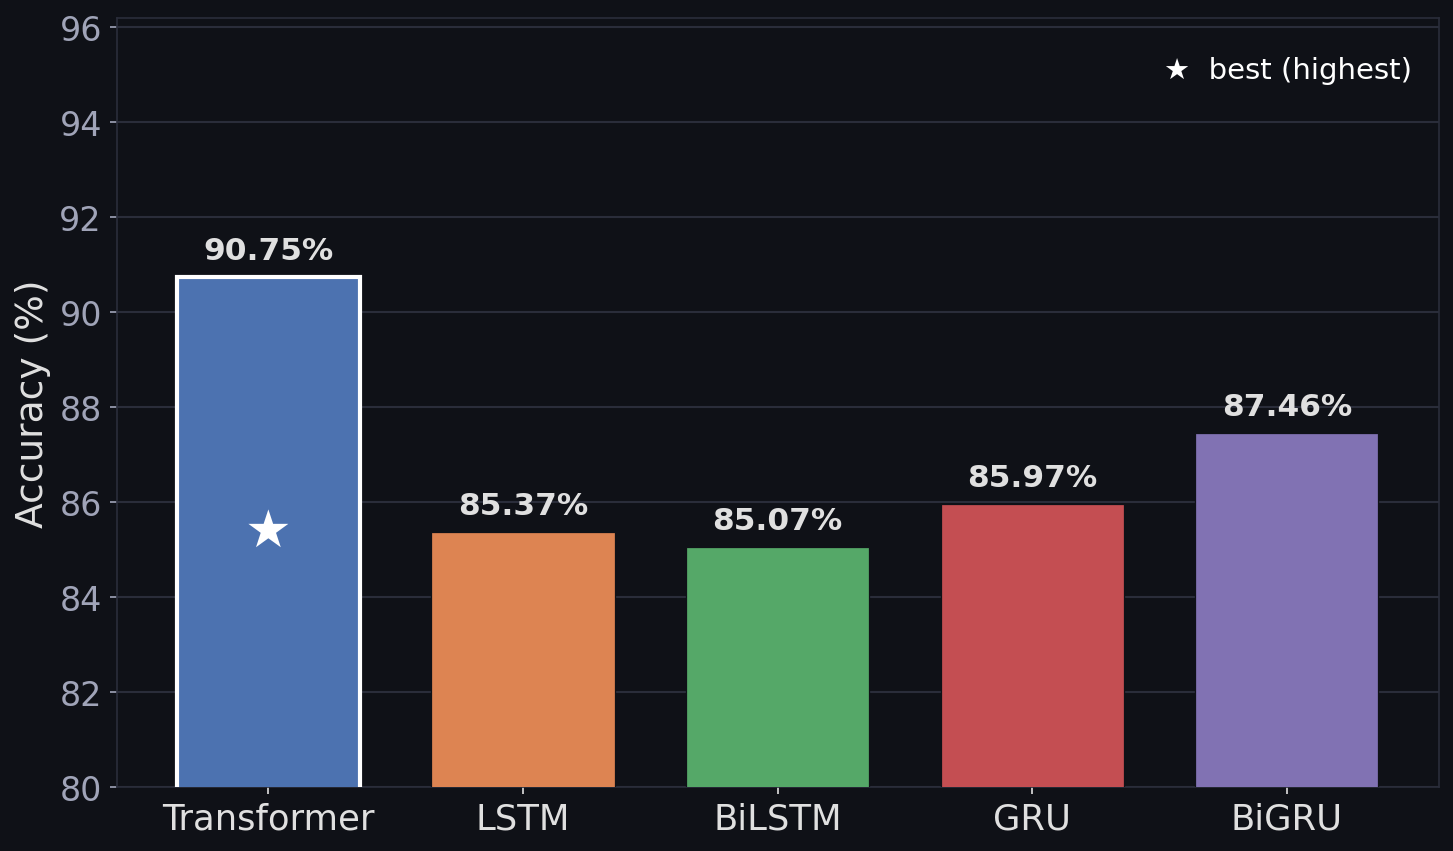
\includegraphics[width=0.48\textwidth]{figures/gloss-recognition/accuracy-validation.png}\hfill
  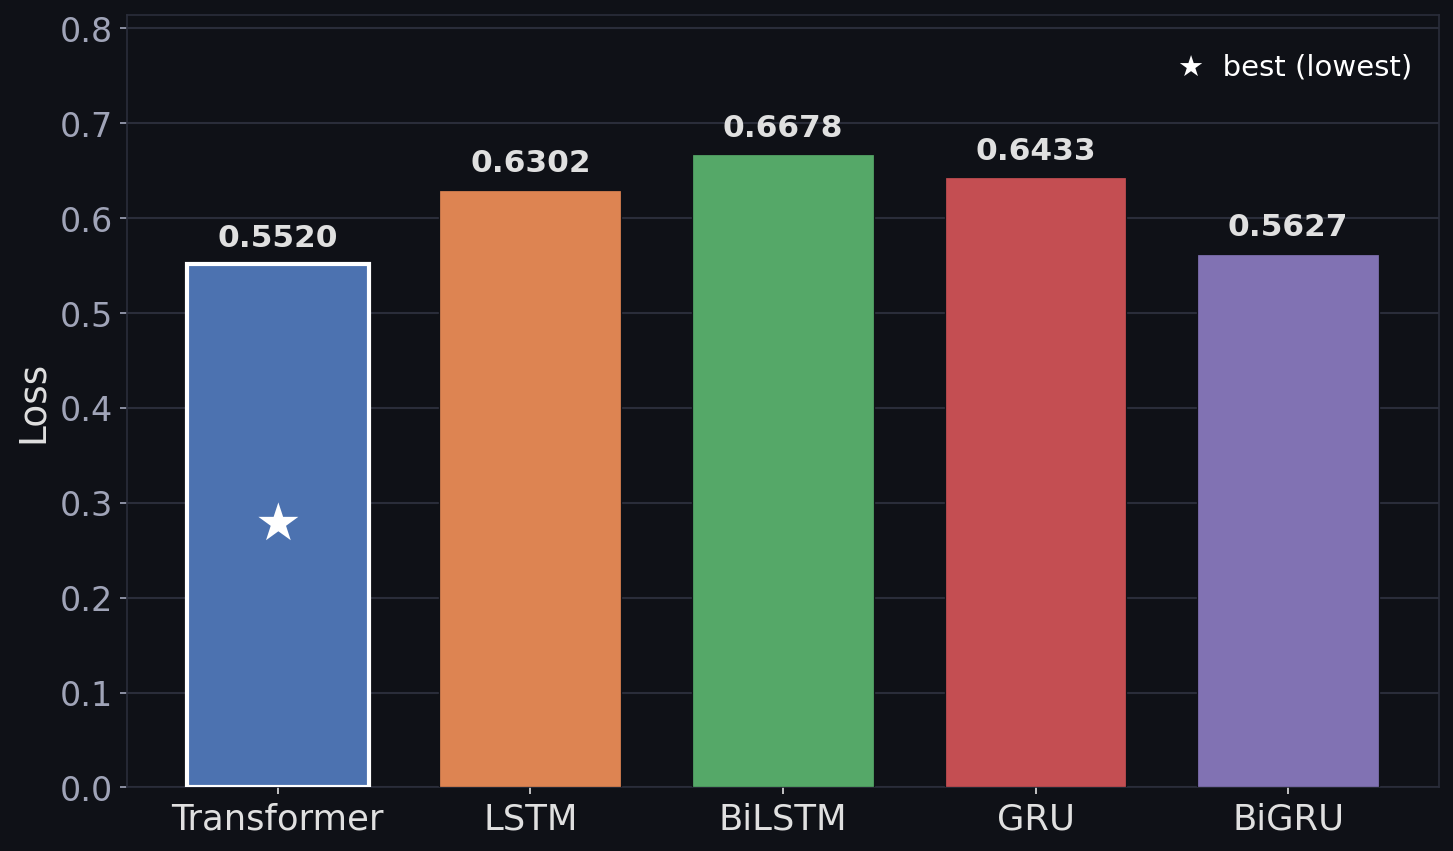
\includegraphics[width=0.48\textwidth]{figures/gloss-recognition/loss-validation.png}
  \caption{Validation accuracy (left) and validation loss (right) across the
  five benchmarked temporal encoders.}
  \label{fig:accuracy-loss}
\end{figure}

\begin{figure}[htbp]
  \centering
  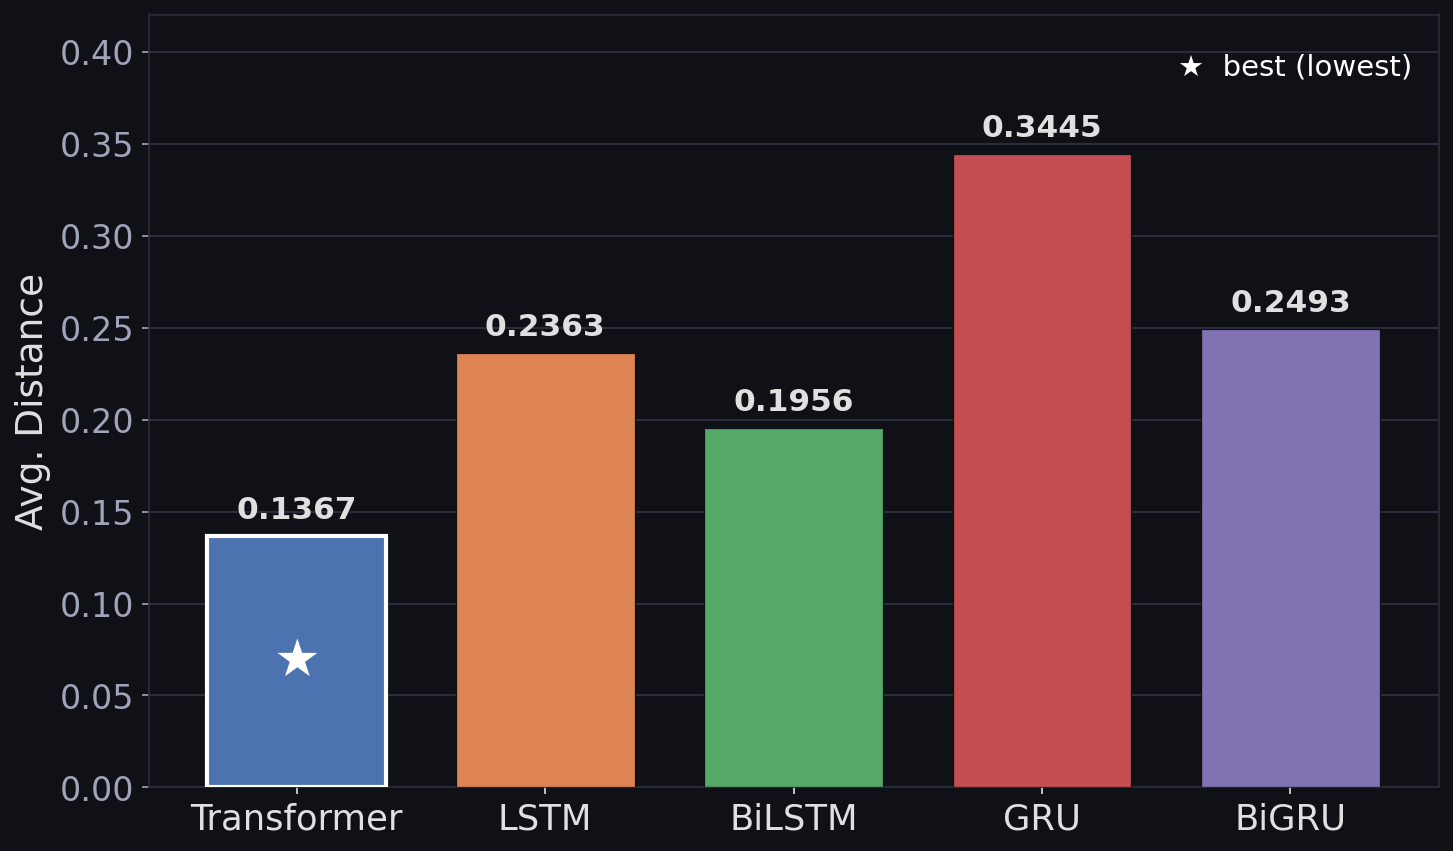
\includegraphics[width=0.32\textwidth]{figures/gloss-recognition/train-positive-distance.png}\hfill
  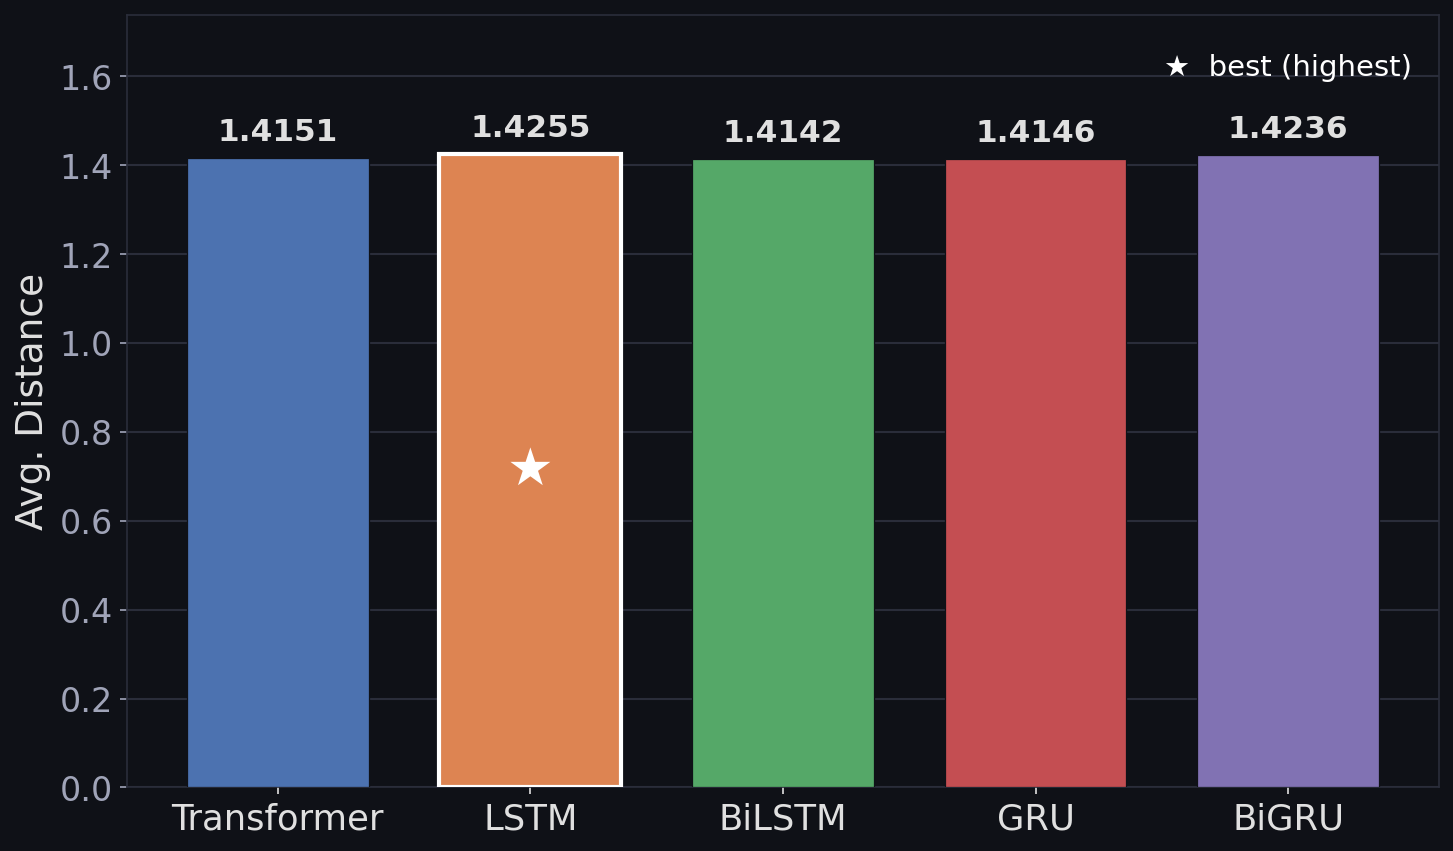
\includegraphics[width=0.32\textwidth]{figures/gloss-recognition/train-negative-distance.png}\hfill
  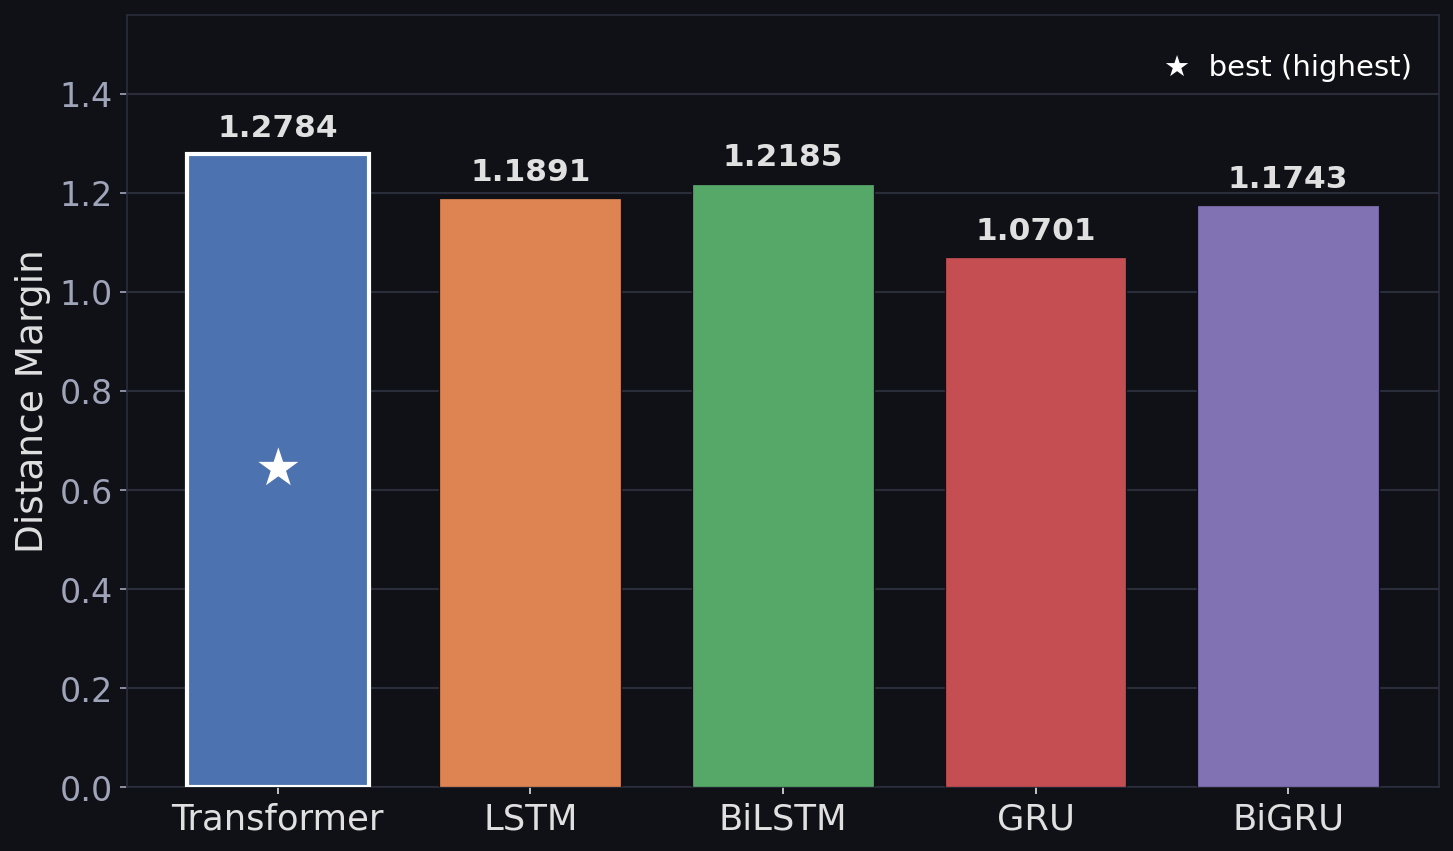
\includegraphics[width=0.32\textwidth]{figures/gloss-recognition/train-distance-margin.png}
  \caption{Positive pair distance, negative pair distance, and distance margin
  (train vs.\ validation) across the five benchmarked temporal encoders.}
  \label{fig:distance-metrics}
\end{figure}

As illustrated in Figures~\ref{fig:accuracy-loss} and~\ref{fig:distance-metrics},
the Transformer encoder achieves the strongest performance across the majority
of reported metrics, attaining the highest 1-NN accuracy (\textbf{90.75\%}),
lowest composite loss, largest distance margin, and smallest positive pair
distance. The sole exception is mean negative pair distance, on which the
Transformer is marginally outperformed by the BiGRU and LSTM encoders; this
difference is negligibly small and does not meaningfully affect the overall
ranking. Taken together, these results establish the Transformer as the most
effective temporal encoder within the proposed architecture. All subsequent
analysis is therefore conducted exclusively using the Transformer encoder.

\todo{PLACEHOLDER: Insert the exact 1-NN accuracy, loss, positive/negative pair
distance, and distance margin values for the LSTM, BiLSTM, GRU, and BiGRU
encoders (only the Transformer's 90.75\% accuracy figure was available in the
source report) to complete the comparison table.}

\subsection{Analysis and discussion}
\label{sec:gloss-recognition-discussion}

We next present a deeper analysis of the complete proposed system, using the
Transformer as the temporal encoder. The confusion matrix
(Figure~\ref{fig:confusion-matrix}) shows no systematic inter-class bias -- no
evidence of the model consistently confusing one particular gloss for another.
Instead, observed misclassifications are distributed irregularly across gloss
pairs, suggesting that errors stem from intra-class variability in the input
data rather than structural ambiguity in the embedding space: the same gloss is
frequently executed differently across signers, varying in hand shape,
movement trajectory, and signing pace, reflecting natural coarticulation and
stylistic variation inherent to sign language production. This
signer-induced variability is a well-recognised challenge in isolated sign
recognition and motivates the use of a metric learning objective, better suited
to handling intra-class spread than a fixed softmax classifier.

\begin{figure}[htbp]
  \centering
  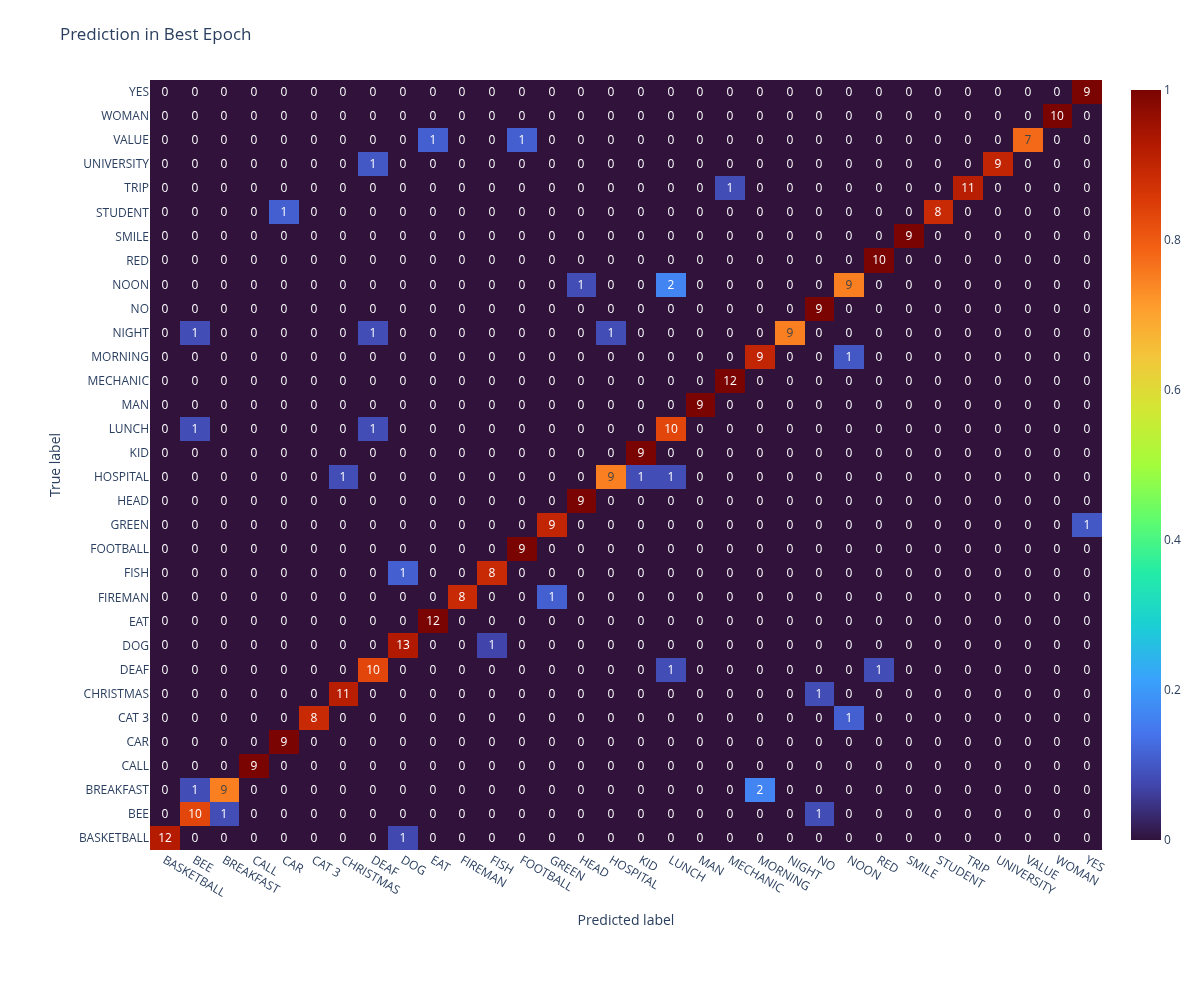
\includegraphics[width=0.6\textwidth]{figures/gloss-recognition/confusion-matrix.png}
  \caption{Confusion matrix over the 32-gloss validation set (Transformer
  encoder).}
  \label{fig:confusion-matrix}
\end{figure}

Per-class recall across all 32 glosses (Figure~\ref{fig:recall-per-class}) shows
that all classes achieve recall exceeding 0.75, demonstrating robust retrieval
performance across the full breadth of the evaluated vocabulary, including both
visually distinctive and potentially ambiguous signs. A substantial number of
glosses attain a perfect recall of 1.0. The absence of any class falling below
the 0.75 threshold is significant, as it suggests the model does not exhibit the
per-class performance collapse common in imbalanced or high-variance
recognition settings, where minority or visually similar classes are frequently
sacrificed in favour of overall accuracy.

\begin{figure}[htbp]
  \centering
  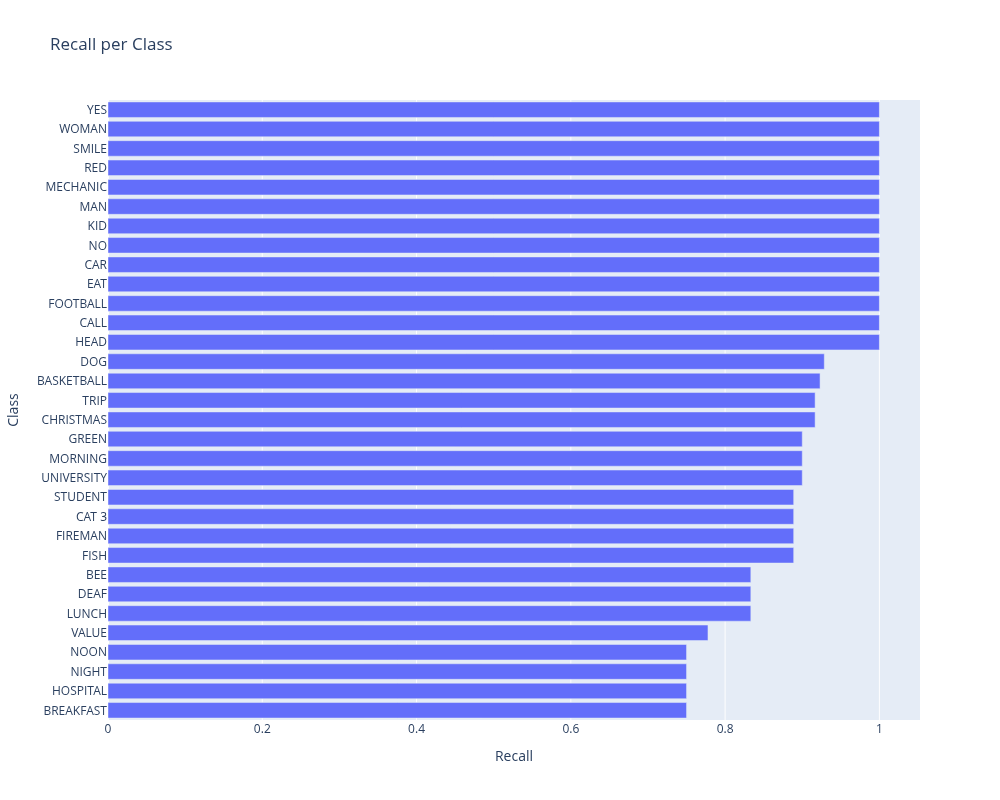
\includegraphics[width=0.6\textwidth]{figures/gloss-recognition/recall-per-class.png}
  \caption{Per-class recall across the 32 evaluated glosses (Transformer
  encoder).}
  \label{fig:recall-per-class}
\end{figure}

We assess the geometric quality of the learned embedding space by visualising
the Transformer's embeddings for both the training and validation sets via
t-SNE (t-Distributed Stochastic Neighbour Embedding), which preserves local
neighbourhood structure and is well-suited to revealing cluster geometry. The
training set embedding space (Figure~\ref{fig:tsne-training}) exhibits
well-defined, non-overlapping clusters -- one per gloss -- with a high degree of
intra-class compactness, confirming that the composite loss has successfully
shaped the embedding space to reflect gloss identity. The validation set
embedding space (Figure~\ref{fig:tsne-validation}) preserves the overall cluster
structure observed during training -- all 32 glosses remain separable -- though
the clusters are noticeably more diffuse, with a degree of inter-class overlap
present at cluster boundaries. This divergence between training and validation
geometry is consistent with the intra-class variability discussed above: the
model has learned a compact representation of the training instances of each
gloss, but unseen signers introduce variation that causes some validation
embeddings to drift toward the boundaries of adjacent clusters. Importantly, the
persistence of globally coherent cluster structure in the validation space
confirms that the model has learned generalisable gloss representations rather
than overfitting to the specific signers present in the training set.

\begin{figure}[htbp]
  \centering
  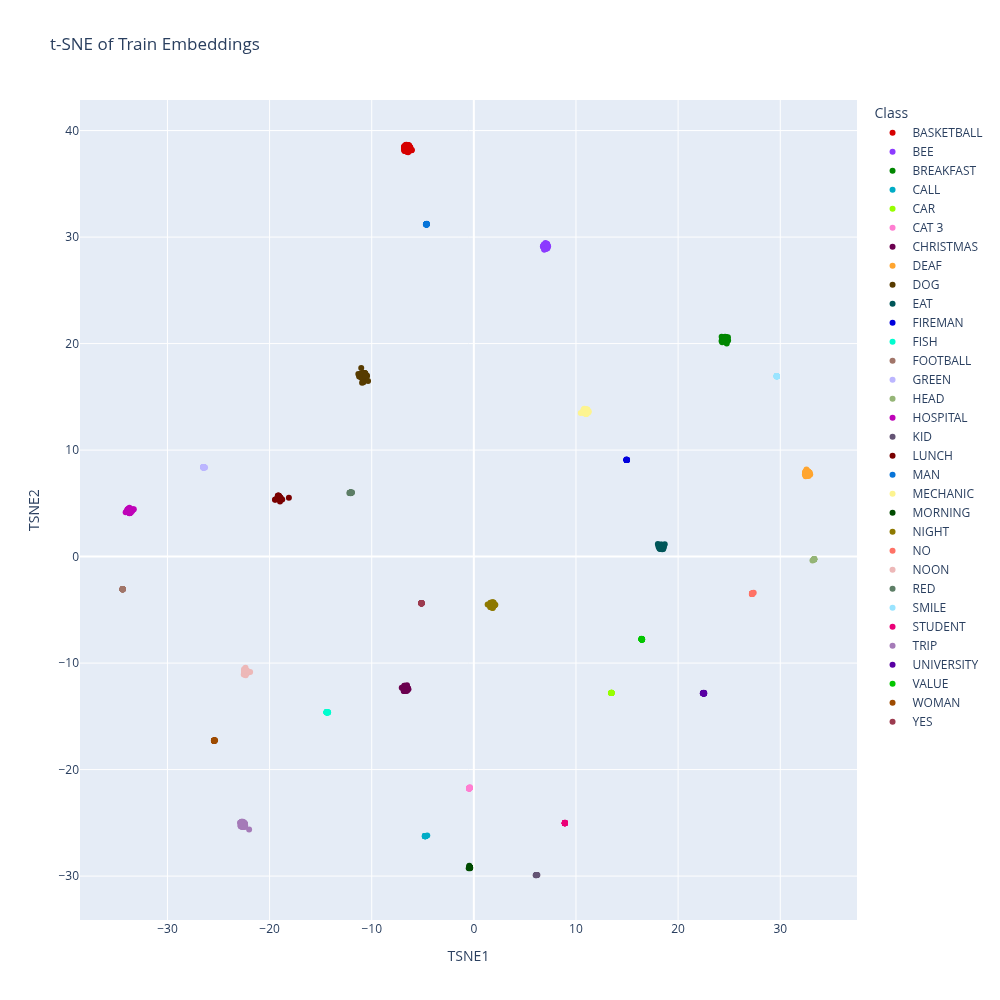
\includegraphics[width=0.48\textwidth]{figures/gloss-recognition/tsne-training.png}\hfill
  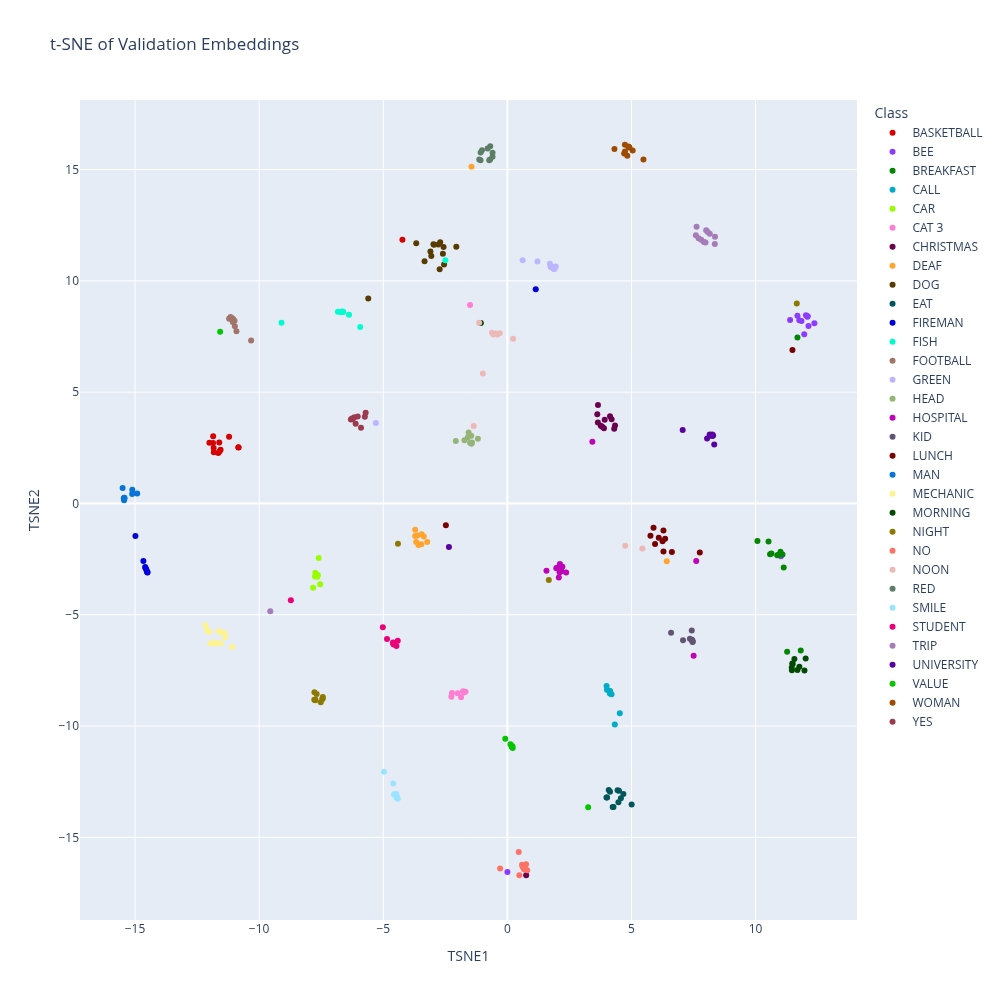
\includegraphics[width=0.48\textwidth]{figures/gloss-recognition/tsne-validation.png}
  \caption{t-SNE visualisation of the learned embedding space on the training
  set (left) and validation set (right).}
  \label{fig:tsne-training}
  \label{fig:tsne-validation}
\end{figure}

Finally, we examine the evolution of mean positive and negative pair distances
under the MS loss over the course of training (Figure~\ref{fig:pos-neg-distances}).
The negative pair distance increases rapidly in the early stages of training and
subsequently stabilises at a consistently high value, with training and
validation curves closely aligned throughout, indicating that the model
reliably learns to separate embeddings of different glosses in a manner that
generalises well to unseen samples. The positive pair distance decreases
steadily over training, reflecting the progressive compaction of within-class
clusters; however, a persistent gap between the training and validation curves
is observed, with validation positive distances remaining consistently higher.
This divergence is a direct manifestation of the intra-class variability
discussed above: while the model successfully compacts the embeddings of
training instances of each gloss, unseen signers in the validation set
introduce execution differences that the model has not been exposed to,
causing their embeddings to be more dispersed within the cluster. This gap thus
quantifies, in embedding-space geometry, the core challenge posed by
signer-dependent variation in sign language recognition.

\begin{figure}[htbp]
  \centering
  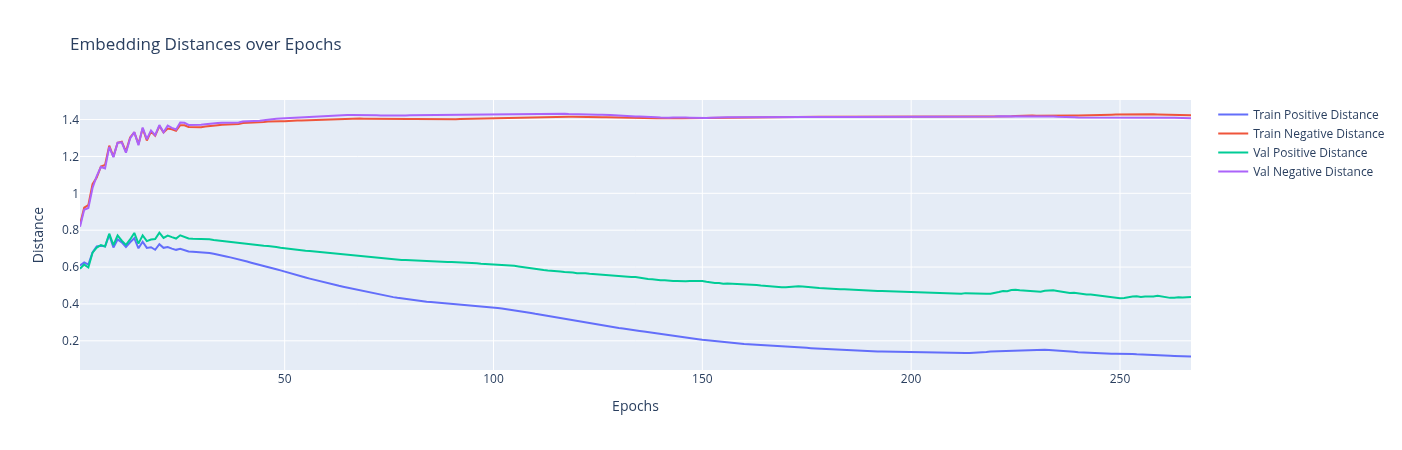
\includegraphics[width=0.6\textwidth]{figures/gloss-recognition/pos-neg-distances.png}
  \caption{Evolution of mean positive and negative pair distances over
  training.}
  \label{fig:pos-neg-distances}
\end{figure}

\subsubsection{Summary}

We have presented a retrieval-based isolated sign language recognition system
for the video-to-gloss task. Starting from raw video, a MediaPipe-based
extraction pipeline produces per-frame skeletal landmark sequences, which are
preprocessed through hand activity checking, temporal interpolation, static
frame removal, Savitzky-Golay smoothing, spatial normalisation, and fixed-length
resampling to 60 frames. The preprocessed sequences are lifted into a
higher-dimensional feature space via a time-distributed projection layer before
being passed to a temporal encoder, benchmarked across five variants. The
Transformer encoder consistently outperforms all recurrent variants across the
majority of evaluated metrics and is selected as the basis for all subsequent
analysis. The encoder is trained under a composite objective combining
Multi-Similarity loss with a reconstruction regularisation term ($\gamma=0.25$),
producing a geometrically structured embedding space in which gloss identity is
reflected by cluster membership, from which a $k$-nearest neighbours classifier
yields the final gloss prediction. Evaluated on a 32-gloss subset of the ASL
Citizen dataset, the system achieves per-class recall exceeding 0.75 across all
glosses, with a substantial number of glosses attaining perfect recall. The
primary limitation identified across all evaluation dimensions is intra-class
variability arising from signer-dependent execution differences, which
manifests as elevated positive pair distances and increased cluster diffusion
for unseen signers.

\subsubsection{Planned extensions}

Several concrete directions for extending the present system target specific
architectural, methodological, and task-scope limitations identified above.

\textbf{Dynamic Time Warping (DTW) at retrieval time.} The current KNN
classifier operates on fixed-length embedding vectors produced by global mean
pooling, which collapses the full temporal structure of the gesture into a
single summary vector. A natural extension is to replace or augment this with
DTW-based sequence similarity, which finds the optimal temporal alignment
between two sequences and is robust to temporal shifts and speed variation --
both common sources of intra-class variability in sign language production.
Unlike Euclidean distance, which aligns sequences by timestamp regardless of
feature values, DTW aligns by content. This extension has a direct
architectural prerequisite: for DTW to produce meaningful alignment distances,
compared sequences must lie in a common, geometrically coherent space, which is
precisely the role of the reconstruction decoder introduced in this chapter --
it constrains the encoder to produce embeddings that remain structurally
grounded in the landmark coordinate space.

\textbf{Soft-DTW as a training objective.} Standard DTW is non-differentiable,
which makes it incompatible with gradient-based training. Soft-DTW
\cite{cuturi2017softdtw} addresses this by replacing the hard minimum over
alignment paths with a soft-minimum over all alignment costs, smoothed via a
temperature parameter $\gamma_{DTW}$ that recovers standard DTW as
$\gamma_{DTW} \to 0$; both its value and gradient can be computed in quadratic
time via dynamic programming, making it tractable as a training loss. We plan
to investigate replacing the MSE reconstruction loss $\mathcal{L}_{rec}$
(Equation~\ref{eq:mse-loss}) with soft-DTW as the decoder objective, training the
decoder -- and by extension the encoder -- under a loss explicitly invariant to
temporal shifts and speed variation.

\textbf{FAISS for scalable retrieval.} The current KNN classifier performs exact
nearest-neighbour search over the full reference embedding set, which scales
linearly with training set size and becomes prohibitive as vocabulary grows. We
plan to replace this with FAISS (Facebook AI Similarity Search)
\cite{johnson2019faiss}, supporting indexing strategies such as IVF (Inverted
File Index) and HNSW (Hierarchical Navigable Small World graphs) that achieve
sublinear retrieval time with controllable accuracy-speed trade-offs; since the
embedding space is L2-normalised and confined to the unit hypersphere, FAISS's
inner-product search mode is directly applicable. This extension is essential
for scaling the system beyond the current 32-gloss benchmark toward a
full-vocabulary deployment.

\todo{PLACEHOLDER: The project repository already contains a live recognition
demo combining the Transformer encoder with FAISS retrieval (commit ``live
recognition Transformer + FAISS''), built after this report was written. Update
this section from planned to implemented work and report its results, or move
the description to Chapter~\ref{chap:educational-platform} if it is presented
there as the live-demo component of the educational platform.}

\textbf{Graph Convolutional Networks for spatial encoding.} The current
preprocessing pipeline flattens per-frame landmark sets into unstructured
vectors, discarding the topological structure of the skeletal graph (see
Section~\ref{sec:video-to-gloss-methods} and \cite{correia2019stgcn}). Graph
Convolutional Networks offer a principled alternative, encoding the landmark
skeleton as a graph with a predefined adjacency matrix reflecting anatomical
connectivity, propagating information along skeletal edges to produce per-node
embeddings explicitly informed by neighbourhood structure. We plan to
investigate GCN-based per-frame encoders as a replacement for the
time-distributed linear projection layer.

\textbf{Quaternion LSTM for rotation-aware temporal encoding.} Three-dimensional
landmark coordinates encode joint positions that are inherently rotational: the
motion of a hand or finger joint is fundamentally a rotation in $SO(3)$ rather
than a translation in $\mathbb{R}^3$. Standard real-valued LSTMs treat these
coordinates as independent scalar features with no inductive bias toward
rotational structure. Quaternion LSTMs operate in the quaternion algebra
$\mathbb{H}$, representing rotations as unit quaternions and performing gating
operations via the Hamilton product, endowing the network with an explicit
structural prior over rotational transformations. We plan to evaluate a
quaternion-LSTM-based temporal encoder as an alternative to the standard LSTM.

\textbf{Continuous, multi-gesture translation via CTC.} The present system
addresses isolated recognition only: each input sequence corresponds to a
single, pre-segmented gloss. Extending toward continuous, unsegmented signing
sequences -- where gloss boundaries are unknown and must be inferred jointly
with gloss identity -- is the subject of
Chapter~\ref{chap:sentence-level-translation}.
